\documentclass[10pt, xcolor=dvipsnames]{beamer}

\usetheme[block=fill]{metropolis}
\usepackage{appendixnumberbeamer}

\usepackage{booktabs}
\usepackage[scale=2]{ccicons}

\usepackage{pgfplots}
\usepgfplotslibrary{dateplot}

\usepackage{mathrsfs}
\usepackage{bbm}
\usepackage{mathtools}
\usepackage{amsmath}
\usepackage{booktabs}
\usepackage{graphicx}
\usepackage[german,ruled]{algorithm2e}
\usepackage{multirow}
\usepackage{tabularx}
\usepackage{float}
\usepackage{epigraph}
\usepackage{soul}
\usepackage[dvipsnames]{xcolor}
\usepackage{listings}
\usepackage[T1]{fontenc}
\usepackage[utf8]{inputenc}
\usepackage{amssymb} % mathfrak + amsfonts + spezielle Symbole
\usepackage{amsxtra} % Weitere Extrasymbole
\usepackage{mathrsfs}
\usepackage{extarrows}
\usepackage{mathrsfs}
\usepackage{textcomp}
\usepackage{stmaryrd}
\usepackage{tabulary}
%\usepackage{color}
\usepackage{mathptmx}
\usepackage[T1]{fontenc}
%\usepackage{caption}

\usepackage{xspace}
\usepackage{xcolor,colortbl}
\usepackage{pifont}% http://ctan.org/pkg/pifont

\newcommand{\cmark}{\ding{51}}%
\newcommand{\xmark}{\ding{55}}%

\newcommand\MyBox[1]{
  \fbox{\lower0.75cm
    \vbox to 1.7cm{\vfil
      \hbox to 1.7cm{\hfil\parbox{1.4cm}{#1}\hfil}
      \vfil}%
  }%
}

\newcommand{\themename}{\textbf{\textsc{metropolis}}\xspace}
\usefonttheme[onlymath]{serif}

\newcolumntype{P}[1]{>{\centering\arraybackslash}p{#1}} %
\newcolumntype{H}[1]{>{\centering\arraybackslash\columncolor{mLightBrown}}p{#1}} %
\newcolumntype{R}[1]{>{\centering\arraybackslash\columncolor{red}}p{#1}} %


\definecolor{airforceblue}{rgb}{0.36, 0.54, 0.66}
\definecolor{cerulean}{rgb}{0.0, 0.48, 0.65}
\definecolor{darkcerulean}{rgb}{0.03, 0.27, 0.49}
\definecolor{mediumpersianblue}{rgb}{0.0, 0.4, 0.65}
\definecolor{mediumelectricblue}{rgb}{0.01, 0.31, 0.59}

\DeclareMathOperator*{\argmax}{arg\,max}
\DeclareMathOperator*{\argmin}{arg\,min}

\title{\large DMC 2020: Prediction of Product Stocks}
\subtitle{\normalsize Data Mining II (FSS2020)}
\author{\scriptsize Rebecca Armbruster \and
	Wei-Yi Chen \and
	Anna Fuchs \and Sang Hyu Hahn
	\and \\Christian Klaus
	\and Jonas Klenk
	\and Jana Pfeffer
	\and Yen-Ting Wang}
\institute{Team abraca-data}
\date{\small{May 5, 2020}}
%

\makeatletter
\setbeamertemplate{title page}{
  \begin{minipage}[b][\paperheight]{\textwidth}
    \centering  % <-- Center here
    \ifx\inserttitlegraphic\@empty\else\usebeamertemplate*{title graphic}\fi
    \vfill%
    \ifx\inserttitle\@empty\else\usebeamertemplate*{title}\fi
    \ifx\insertsubtitle\@empty\else\usebeamertemplate*{subtitle}\fi
    \usebeamertemplate*{title separator}
    \ifx\beamer@shortauthor\@empty\else\usebeamertemplate*{author}\fi
    \ifx\insertinstitute\@empty\else\usebeamertemplate*{institute}\fi
    \vspace*{4mm}
    \ifx\insertdate\@empty\else\usebeamertemplate*{date}\fi
    \vfill
    \vspace*{1mm}
  \end{minipage}
}

\setbeamertemplate{title}{
%  \raggedright%  % <-- Comment here
  \linespread{1.0}%
  \inserttitle%
  \par%
  \vspace*{0.5em}
}
\setbeamertemplate{subtitle}{
%  \raggedright%  % <-- Comment here
  \insertsubtitle%
  \par%
  \vspace*{0.5em}
}
\makeatother

%\captionsetup{font=scriptsize,labelfont=scriptsize,justification=centering,labelformat=empty,width=\textwidth}


\begin{document}	
\setlength\tabcolsep{1.5pt}
\maketitle
%\begin{frame}{Outline}
%\setbeamertemplate{section in toc}[sections numbered]
%\tableofcontents[hideallsubsections]
%\end{frame}
%\section{Introduction}
\begin{frame}{Data}
\begin{centering}
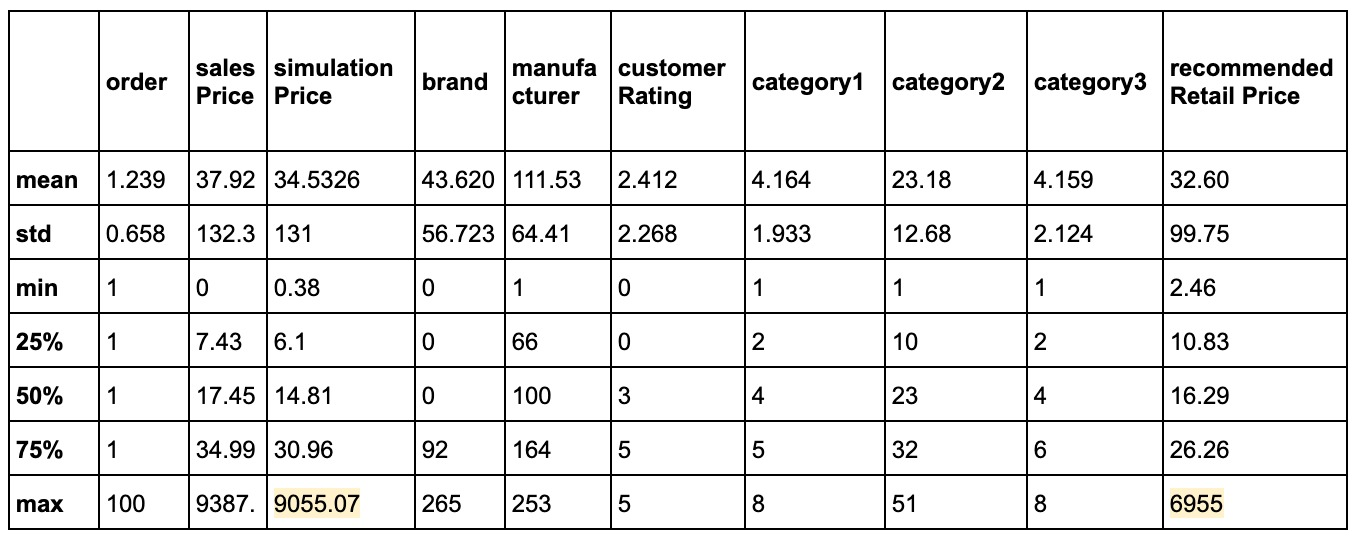
\includegraphics[width=\textwidth]{data.jpg}
\end{centering}
\end{frame}

\begin{frame}{First Approach}
\alert{Methods employed}
        \begin{itemize}
	\item Holt Winter
	\item Random Forest
	\item LSTM
        \end{itemize}
\alert{General data preparation for time series analysis}
\begin{itemize}
	\item Aggregate to items sold per day per item.
	\item Replace missing days with zeros.
\end{itemize}
\end{frame}

\begin{frame}{Holt Winter}
\begin{figure}
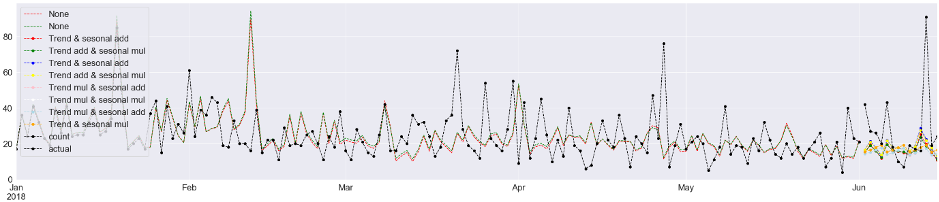
\includegraphics[width=\textwidth]{holt.png}
\caption{\scriptsize Forecasting sales of item 7798 with both additive and multiplicative seasonality.}
\end{figure}

\end{frame}

\begin{frame}{Random Forest}
\begin{itemize}
\item Training data is lagged to create features. 
\item Actual time series as target.
\end{itemize}
\begin{table}
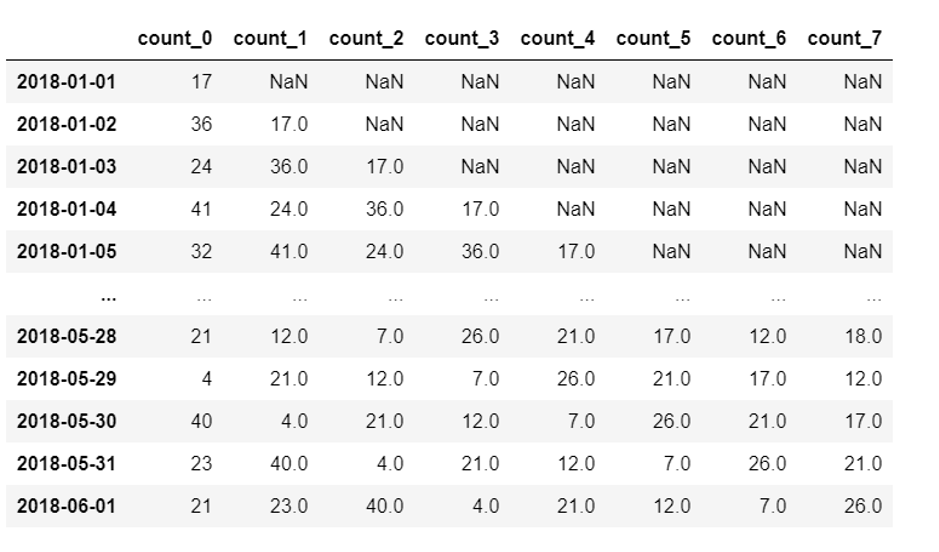
\includegraphics[width=.9\textwidth]{randomforestdata.png}
\caption{Example training data.}
\end{table}

\end{frame}

\begin{frame}{Random Forest}
\begin{figure}
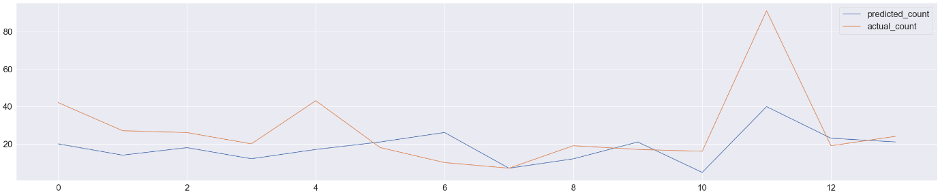
\includegraphics[width=\textwidth]{rf.png}
\caption{Random Forest prediction and actual for item 7798.}
\end{figure}
\alert{Performance compared to baseline:}\\[2px]
Perfect Result: 7895975.87\\
Random Forest: -1,359,513.29\\
Baseline 2: -1,672,504.21\\
Baseline 1: -3,727,365.60\\

\end{frame}

\begin{frame}{LSTM}
\begin{footnotesize}
\begin{itemize}
	\item Generate time series data with 14 lags.
	\item Parameters: activation='relu', dropout(0.15), dense(1), optimizer='adam', loss='mse', shuffle = False, verbose = 1
\end{itemize}
\end{footnotesize}
\begin{figure}
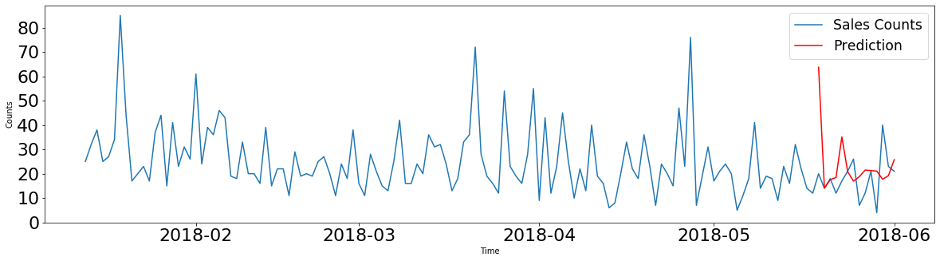
\includegraphics[width=.8\textwidth]{lstm1.png}
\vspace{-12px}
\caption{\tiny Prediction for item 7798 for the last 14 days in training dataset with 500 epochs. Loss: 0.033}
\end{figure}
\vspace{-18px}
\begin{figure}
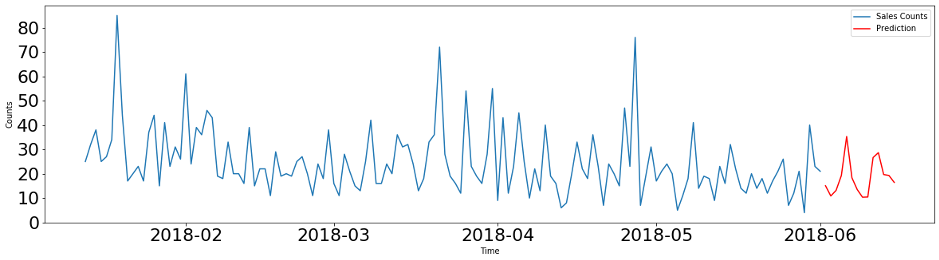
\includegraphics[width=.8\textwidth]{lstm2.png}
\vspace{-12px}
\caption{\tiny Prediction for item 7798 for the last 14 days in training dataset with 150 epochs. Loss: 0020}
\end{figure}

\end{frame}


\begin{frame}{Next Steps}
        \begin{itemize}
         \item Generate good features
         \item Check for seasonality
        \end{itemize}
\end{frame}

\begin{frame}{Feature Generation}
        \begin{itemize}
	\item Purchase time in various dimensions (weekday/day of the month/month/hour/calendar week)
	\item Discount from Recommended Retail Price to Sales Price (absolute/relative)
        \end{itemize}
\begin{figure}
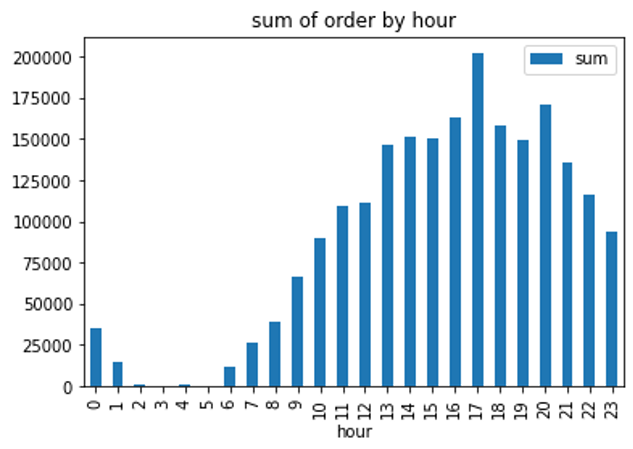
\includegraphics[width=.7\textwidth]{orderbyhour.png}
\end{figure}
\end{frame}

\begin{frame}{Promotion Flag}
\begin{itemize}
	\item Add a promotion flag to orders if an item was promoted that day.
	\begin{itemize}
	\item[$\rightarrow$] Promotions in Info.csv are only available for the future
	\end{itemize}
	\item Explore ways to identify promotions in the orders data as outliers
	\begin{itemize}
		\item[$\rightarrow$] Use IQR as in the lectures
		\item[$\rightarrow$] Use modified IQR $(Median + 2*IQR[25, 90])$
	\end{itemize}
\end{itemize}
\end{frame}


\begin{frame}{Promotion Flag}
\begin{figure}
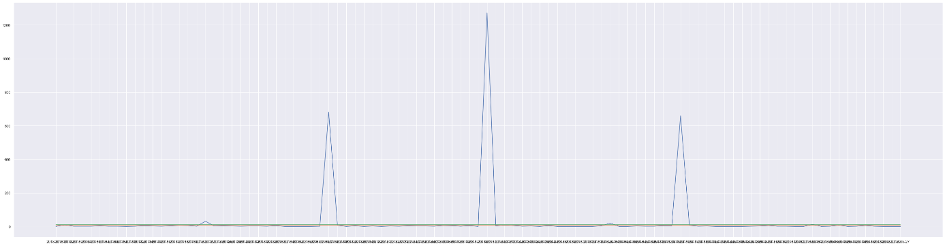
\includegraphics[width=.75\textwidth]{prom1.png}
\end{figure}
\begin{figure}
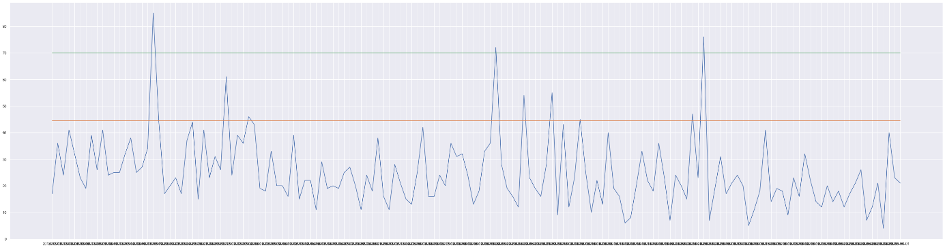
\includegraphics[width=.75\textwidth]{prom2.png}
\end{figure}
\begin{figure}
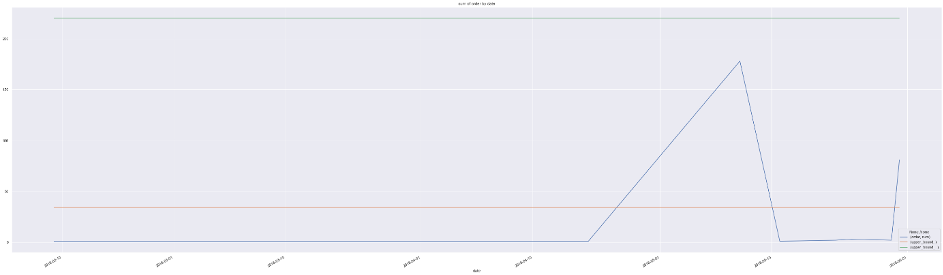
\includegraphics[width=.75\textwidth]{prom3.png}
\end{figure}
\end{frame}

\begin{frame}{Seasonality Check}
\begin{figure}
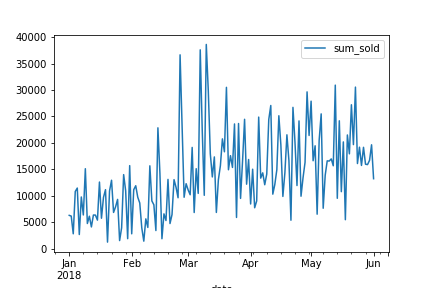
\includegraphics[width=.8\textwidth]{season.png}
\caption{Seasonality.}
\end{figure}
\end{frame}

\begin{frame}{Questions}
        \begin{itemize}
         \item
        \end{itemize}
\end{frame}


\end{document}